\chapter{HH4b: Results}
\label{chap:seven}

\section{Results\label{sec:Results}}

Upper limits at 95\% confidence level are set
on the product of the production cross section and the branching
fractions $\sigma(\Pp\Pp\to\PX) \mathcal{B}(\PX\to\bbbar\bbbar)$.
They are obtained using the profile likelihood as a test
statistic~\cite{ATLASCMSComb}. The systematic uncertainties are
treated as nuisance parameters and are profiled in the minimization of
the negative of the logarithm of the profile likelihood ratio and the
distributions of the likelihood ratio are calculated using the
asymptotic approximation~\cite{AsympCLs} of the procedure reported in
Refs.~\cite{CLS1,CLS2}.

As shown in Fig.~\ref{fig:RadionLimitFULL}, left, a narrow radion with
mass between 1000 and 2600 GeV is excluded at 95\% confidence level
for $\LambdaR=3\TeV$.  Narrow bulk graviton for $k/\overline{\Mpl} =
0.5$ is excluded at 95\% confidence level only for masses between 1000
and 1200 GeV, as shown in Fig.~\ref{fig:GravitonLimitFULL}, right.
The deviation in observed limit at 1300 and 1500  GeV resonance masses
is driven by an upward fluctuation of data over the background prediction at
$\mred \sim$1400 GeV, as can be seen in Fig.~\ref{fig:TTmjj}, middle
row.

The expected limits are reported in Tables~\ref{tab:ExpLimRad} and
\ref{tab:ExpLimBG} for radions and bulk gravitons of different assumed
masses, respectively. The upper limits range from 4.94 to 0.19 fb for the bulk
graviton and from 9.74 to 0.29 fb for the radion for the mass
range $1$--$3$\TeV.

\begin{figure}[!htb]
	\centering
	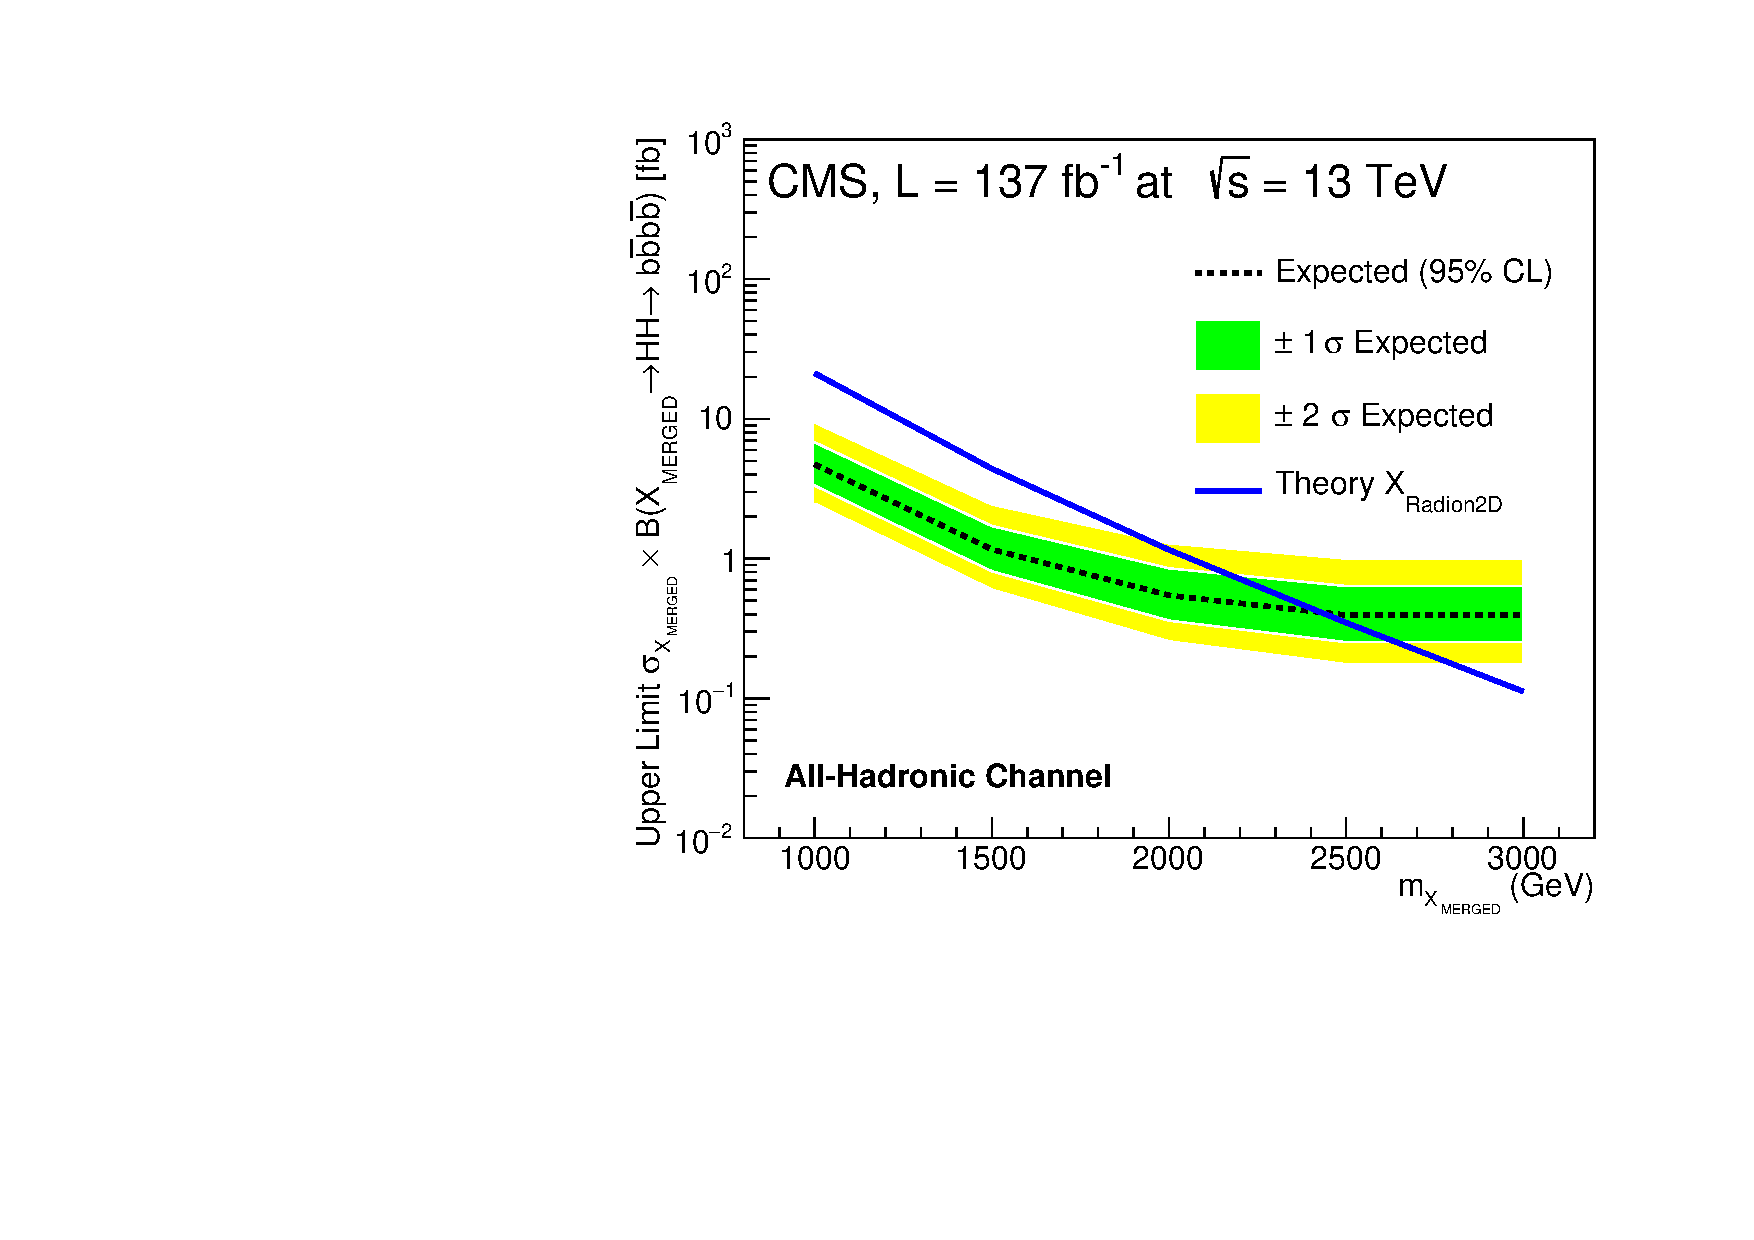
\includegraphics[width=0.5\textwidth]{Figures/limits_combine_137fb_dak8MDHbb_signalsAll_RadNar_MERGED.pdf}
	\caption{Full Run 2 Radion Limit for 1$+$1 using the Deep AK8 Mass Decorrelated Hbb Tagger.}
	\label{fig:RadionLimitMerged}
\end{figure}

\begin{figure}[!htb]
	\centering
	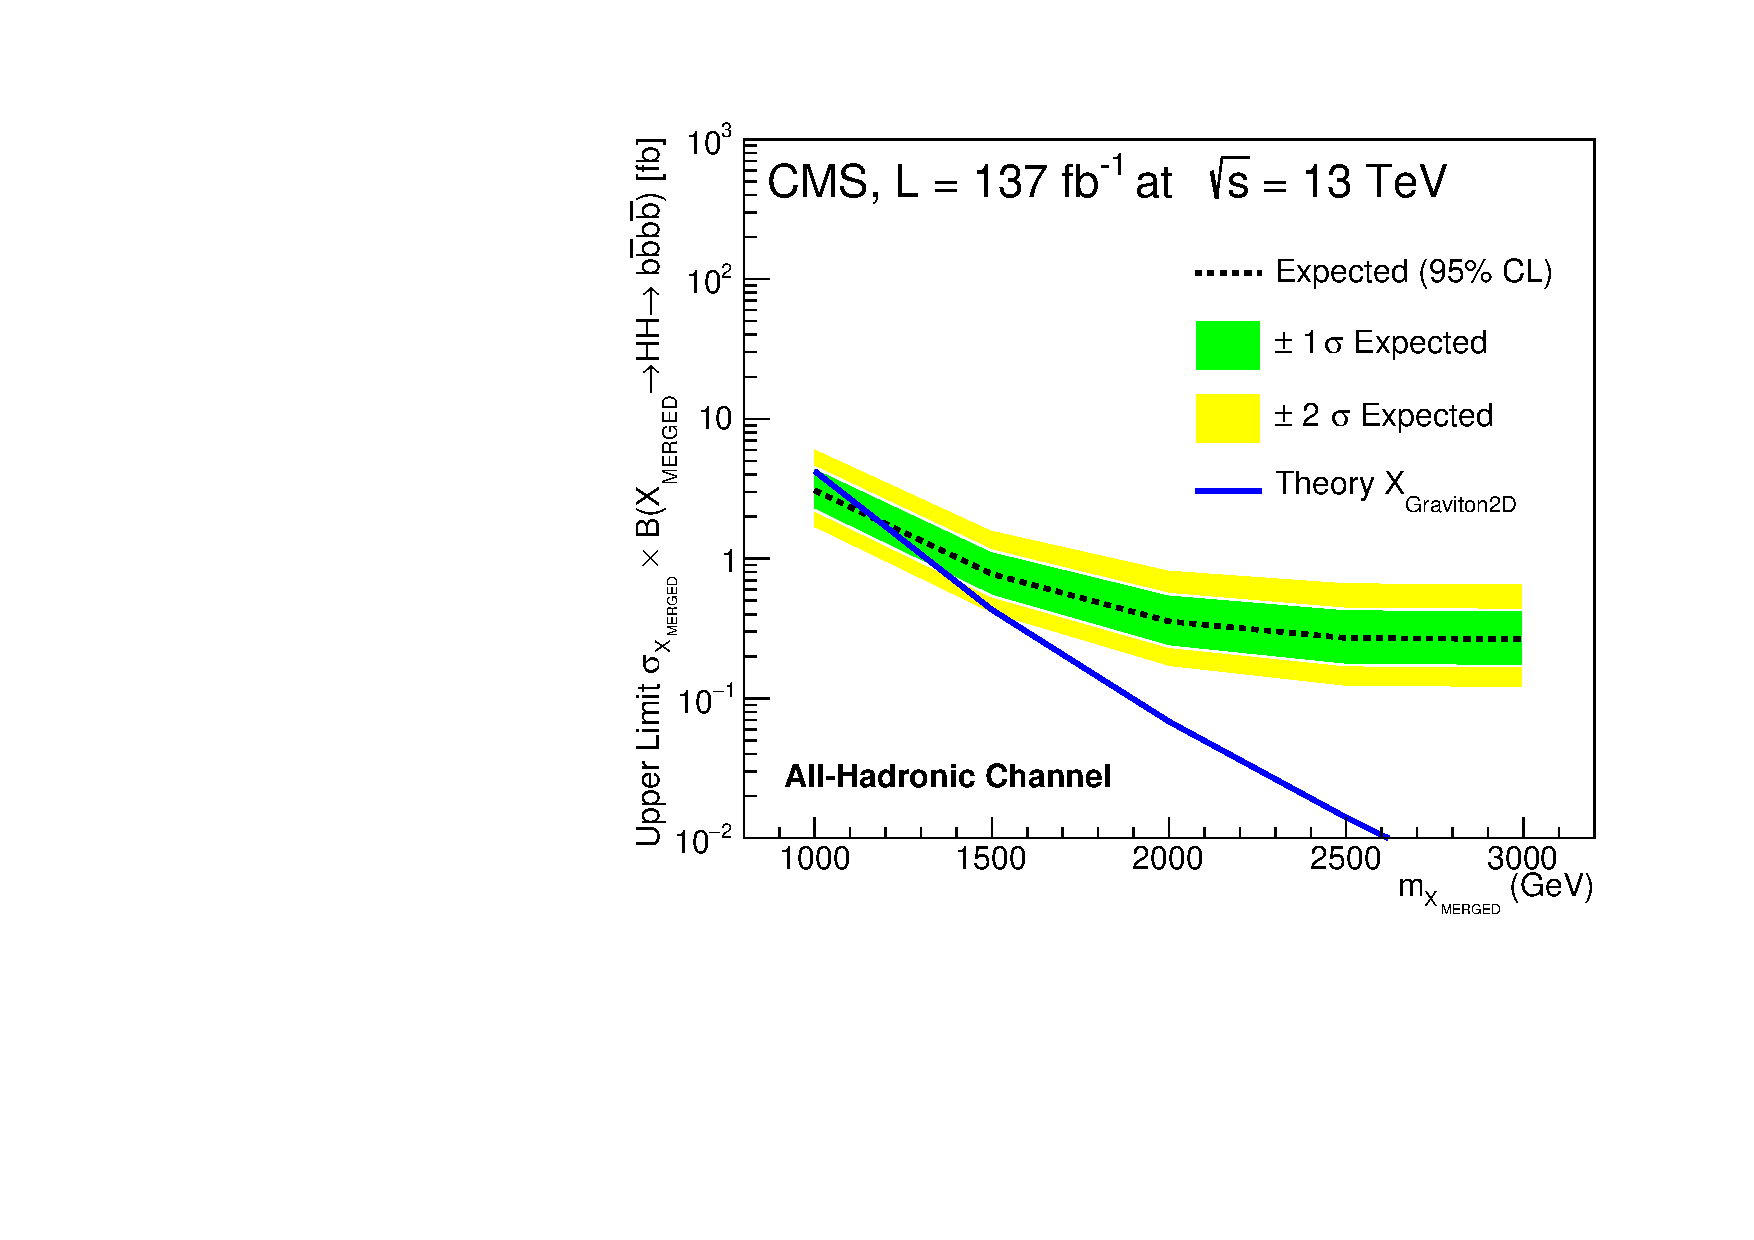
\includegraphics[width=0.5\textwidth]{Figures/limits_combine_137fb_dak8MDHbb_signalsAll_GravNar_MERGED.pdf}
	\caption{Full Run 2 Graviton Limit for 1$+$1 using the Deep AK8 Mass Decorrelated Hbb Tagger.}
	\label{fig:GravitonLimitMerged}
\end{figure}

\begin{figure}[!htb]
	\centering
	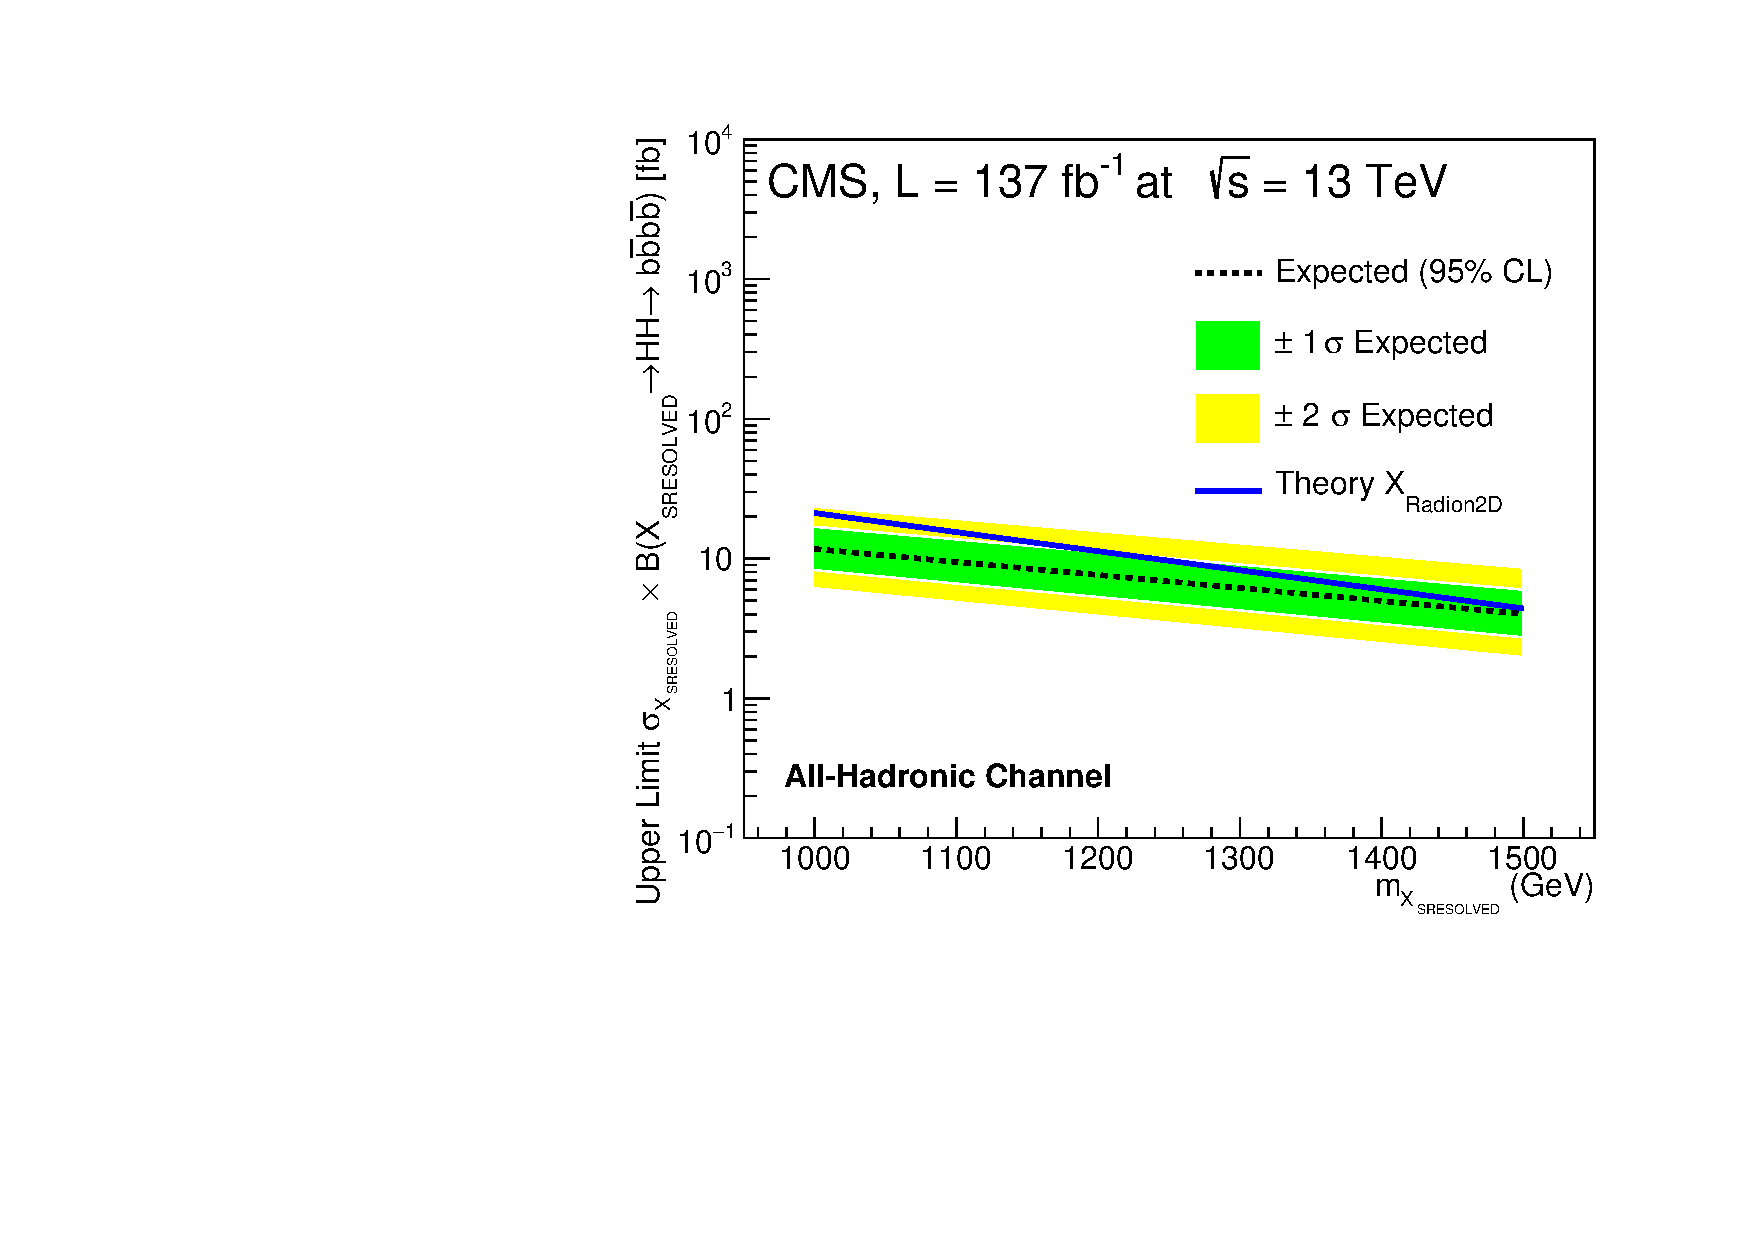
\includegraphics[width=0.5\textwidth]{Figures/limits_combine_137fb_dak8MDHbb_signalsAll_RadNar_SRESOLVED.pdf}
	\caption{Full Run 2 Radion Limit for 2$+$1 using the Deep AK8 Mass Decorrelated Hbb Tagger.}
	\label{fig:RadionLimitSResolved}
\end{figure}

\begin{figure}[!htb]
	\centering
	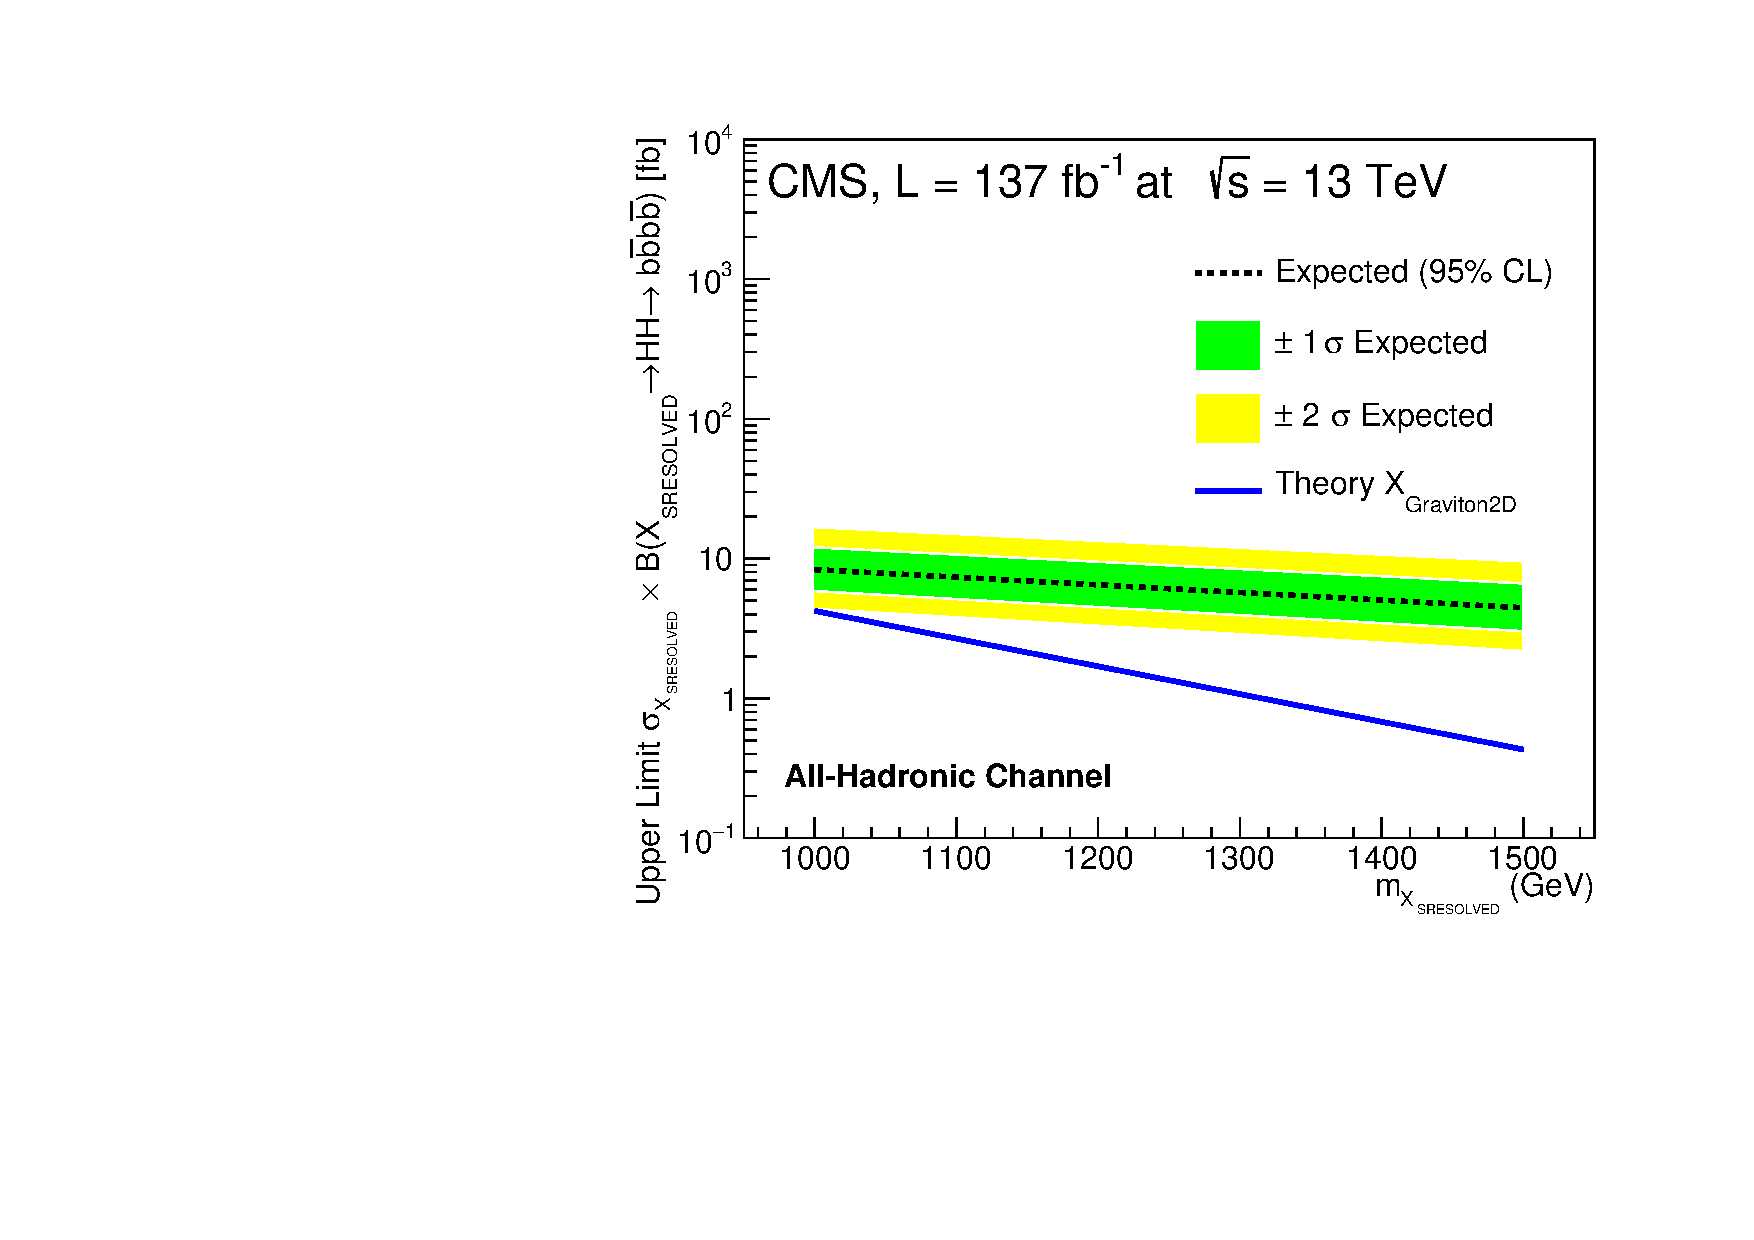
\includegraphics[width=0.5\textwidth]{Figures/limits_combine_137fb_dak8MDHbb_signalsAll_GravNar_SRESOLVED.pdf}
	\caption{Full Run 2 Graviton Limit for 2$+$1 using the Deep AK8 Mass Decorrelated Hbb Tagger.}
	\label{fig:GravitonLimitSResolved}
\end{figure}

\begin{figure}[!htb]
	\centering
	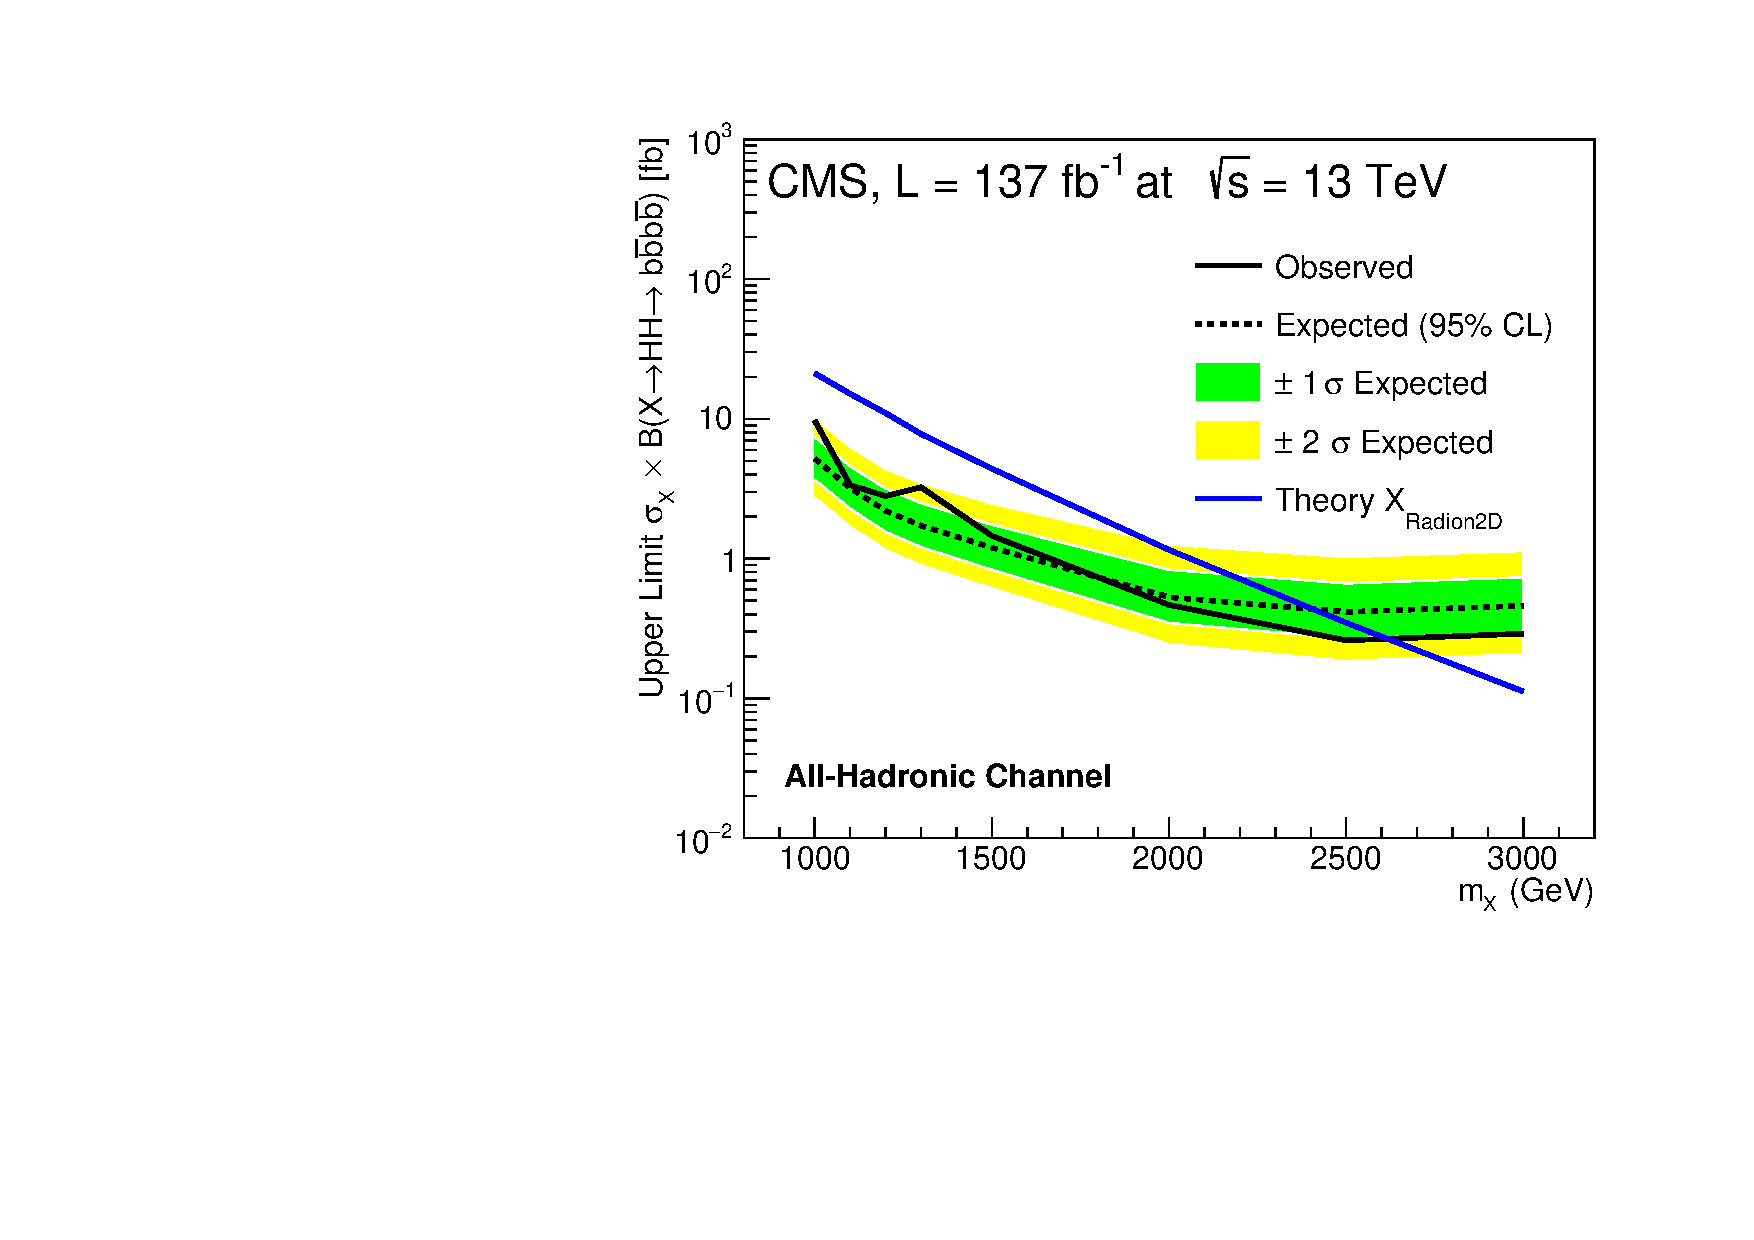
\includegraphics[width=0.45\textwidth]{Figures/limits_combine_137fb_dak8MDHbb_signalsAll_RadNar_2x2.pdf}
        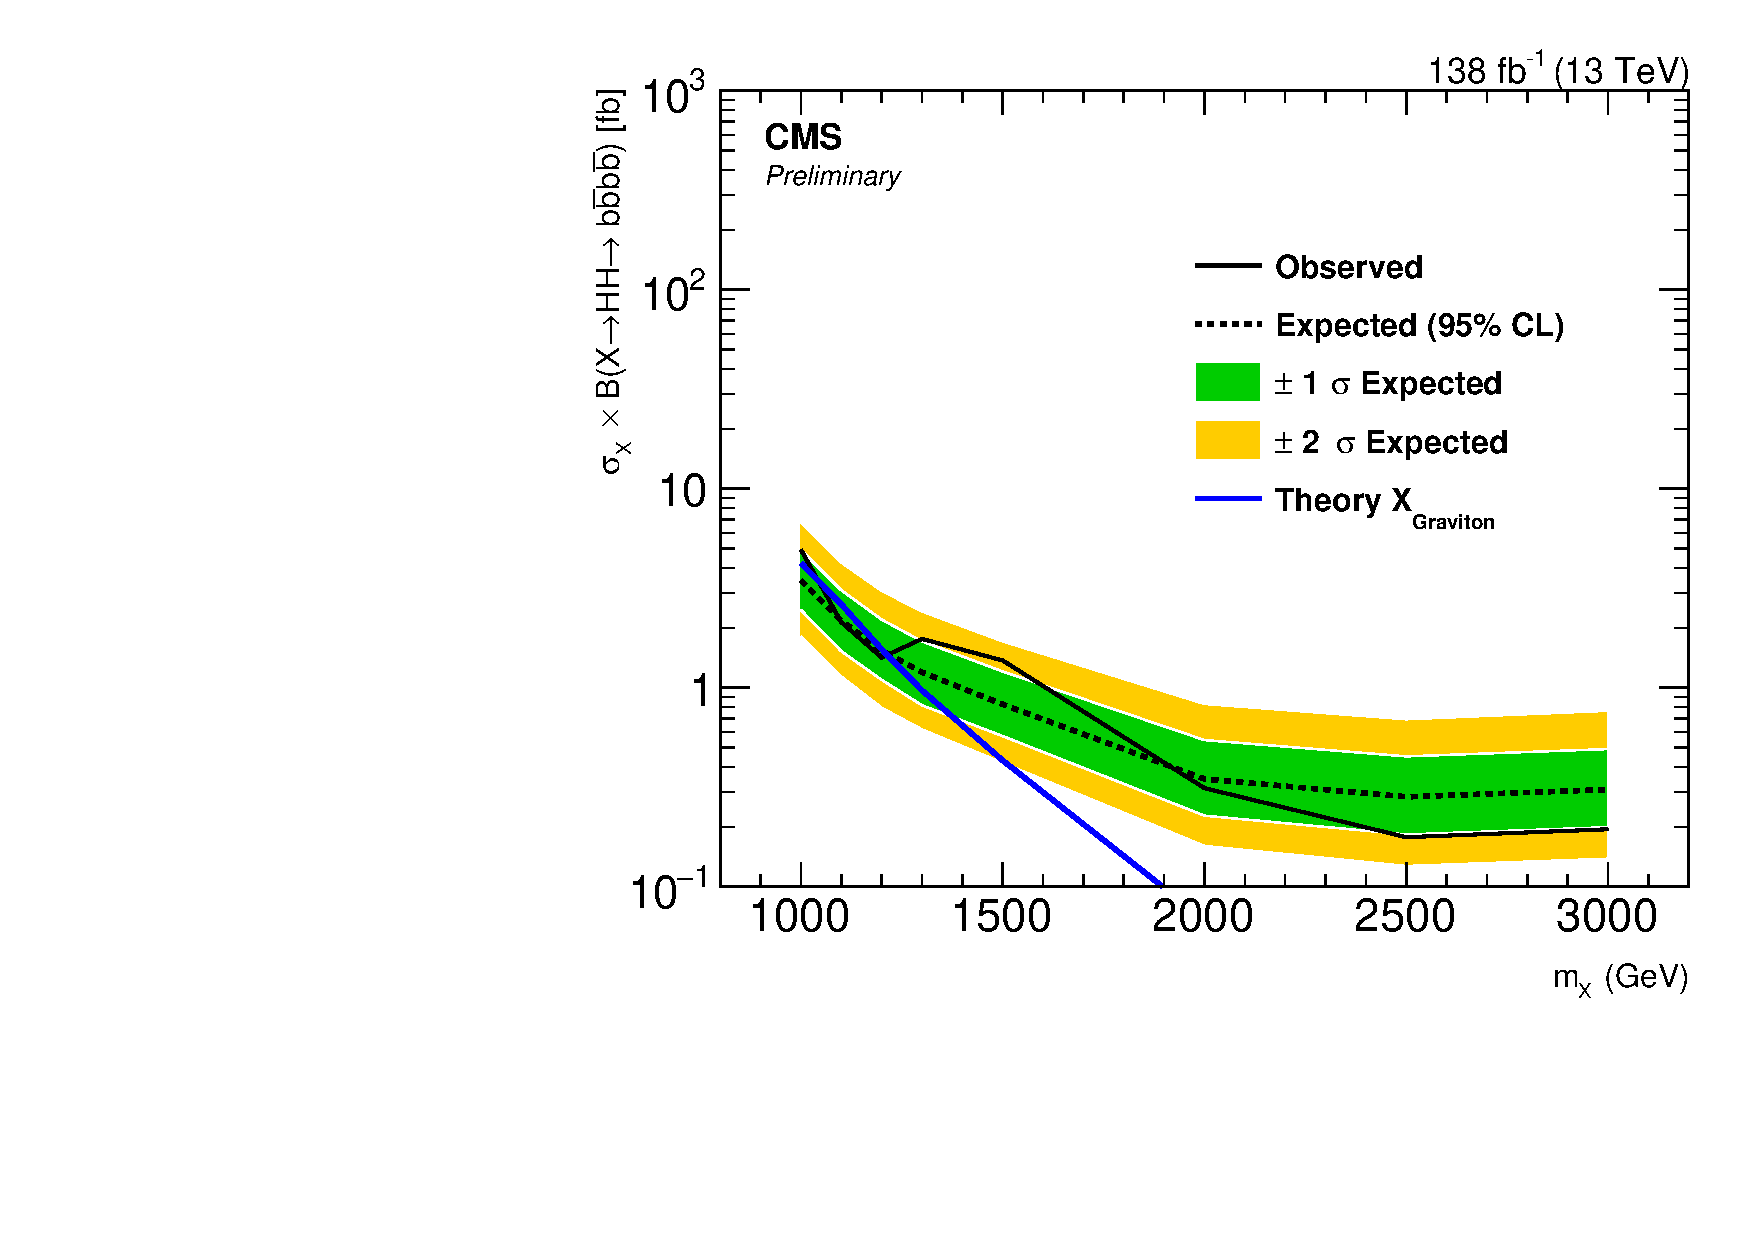
\includegraphics[width=0.45\textwidth]{Figures/limits_combine_137fb_dak8MDHbb_signalsAll_GravNar_2x2.pdf}
        \caption{Upper limits at 95\% confidence level on
        $\sigma(\Pp\Pp\to\PX) \mathcal{B}(\PX\to\bbbar\bbbar)$
        for the narrow spin-0 radion (left) and
        the spin-2 bulk graviton (right) models.  The predicted theoretical
        cross sections for the narrow radion and bulk graviton are also
        shown.}
	\label{fig:RadionLimitFULL}
 	\label{fig:GravitonLimitFULL}
\end{figure}

\begin{table}[h]
	\begin{center}
	\caption{Radion observed 95\% CL exclusion limits.}
	\label{tab:ExpLimRad}
	\begin{tabular}{c c c c c c c } 
	 \hline
	   Mass& Obs. & Exp. lim.& $+$Exp (68\%)& $-$Exp (68\%)& $+$Exp (95\%)& $-$Exp (95\%)\\
	   (GeV) & (fb) & (fb) & (fb) & (fb)& (fb)& (fb) \\
	\hline
	 1000 & 9.74 & 5.12 & 7.41 & 3.68 & 10.26 & 2.74 \\
	 1100 & 3.37 & 3.20 & 4.58 & 2.28 & 6.31 & 1.69 \\
	 1200 & 2.80 & 2.20 & 3.18 & 1.55 & 4.40 & 1.15 \\
	 1300 & 3.24 & 1.72 & 2.50 & 1.21 & 3.5 & 0.89 \\
	 1500 & 1.46 & 1.10 & 1.75 & 0.83 & 2.48 & 0.61 \\
	 2000 & 0.47 & 0.53 & 0.83 & 0.34 & 1.26 & 0.24 \\
	 2500 & 0.26 & 0.42 & 0.66 & 0.26 & 1.02 & 0.18 \\
	 3000 & 0.29 & 0.46 & 0.74 & 0.29 & 1.13 & 0.20 \\ 
	 \hline
	\end{tabular}
	\end{center}
	\end{table}
	
	\begin{table}[h]
	\begin{center}
	\caption{Graviton observed 95\% CL exclusion limits. }
	\label{tab:ExpLimBG}
	\begin{tabular}{c c c c c c c } 
	 \hline
	 Mass& Obs. & Exp. lim.& $+$Exp (68\%)& $-$Exp (68\%)& $+$Exp (95\%)& $-$Exp (95\%)\\
	 (GeV) & (fb) & (fb) & (fb) & (fb)& (fb)& (fb) \\
	\hline
	 1000 & 4.94 & 3.47 & 4.93 & 2.46 & 6.82 & 1.81 \\
	 1100 & 2.13 & 2.12 & 3.10 & 1.52 & 4.26 & 1.14 \\
	 1200 & 1.42 & 1.54 & 2.20 & 1.10 & 3.07 & 0.79 \\
	 1300 & 1.76 & 1.20 & 1.71 & 0.82 & 2.42 & 0.62 \\
	 1500 & 1.37 & 0.83 & 1.21 & 0.57 & 1.71 & 0.42 \\
	 2000 & 0.31 & 0.35 & 0.55 & 0.23 & 0.83 & 0.16 \\
	 2500 & 0.18 & 0.28 & 0.45 & 0.18 & 0.69 & 0.13 \\
	 3000 & 0.19 & 0.31 & 0.49 & 0.20 & 0.77 & 0.14 \\
	 \hline
	\end{tabular}
	\end{center}
\end{table}
\clearpage

\begin{figure}[!htb]
	\centering
	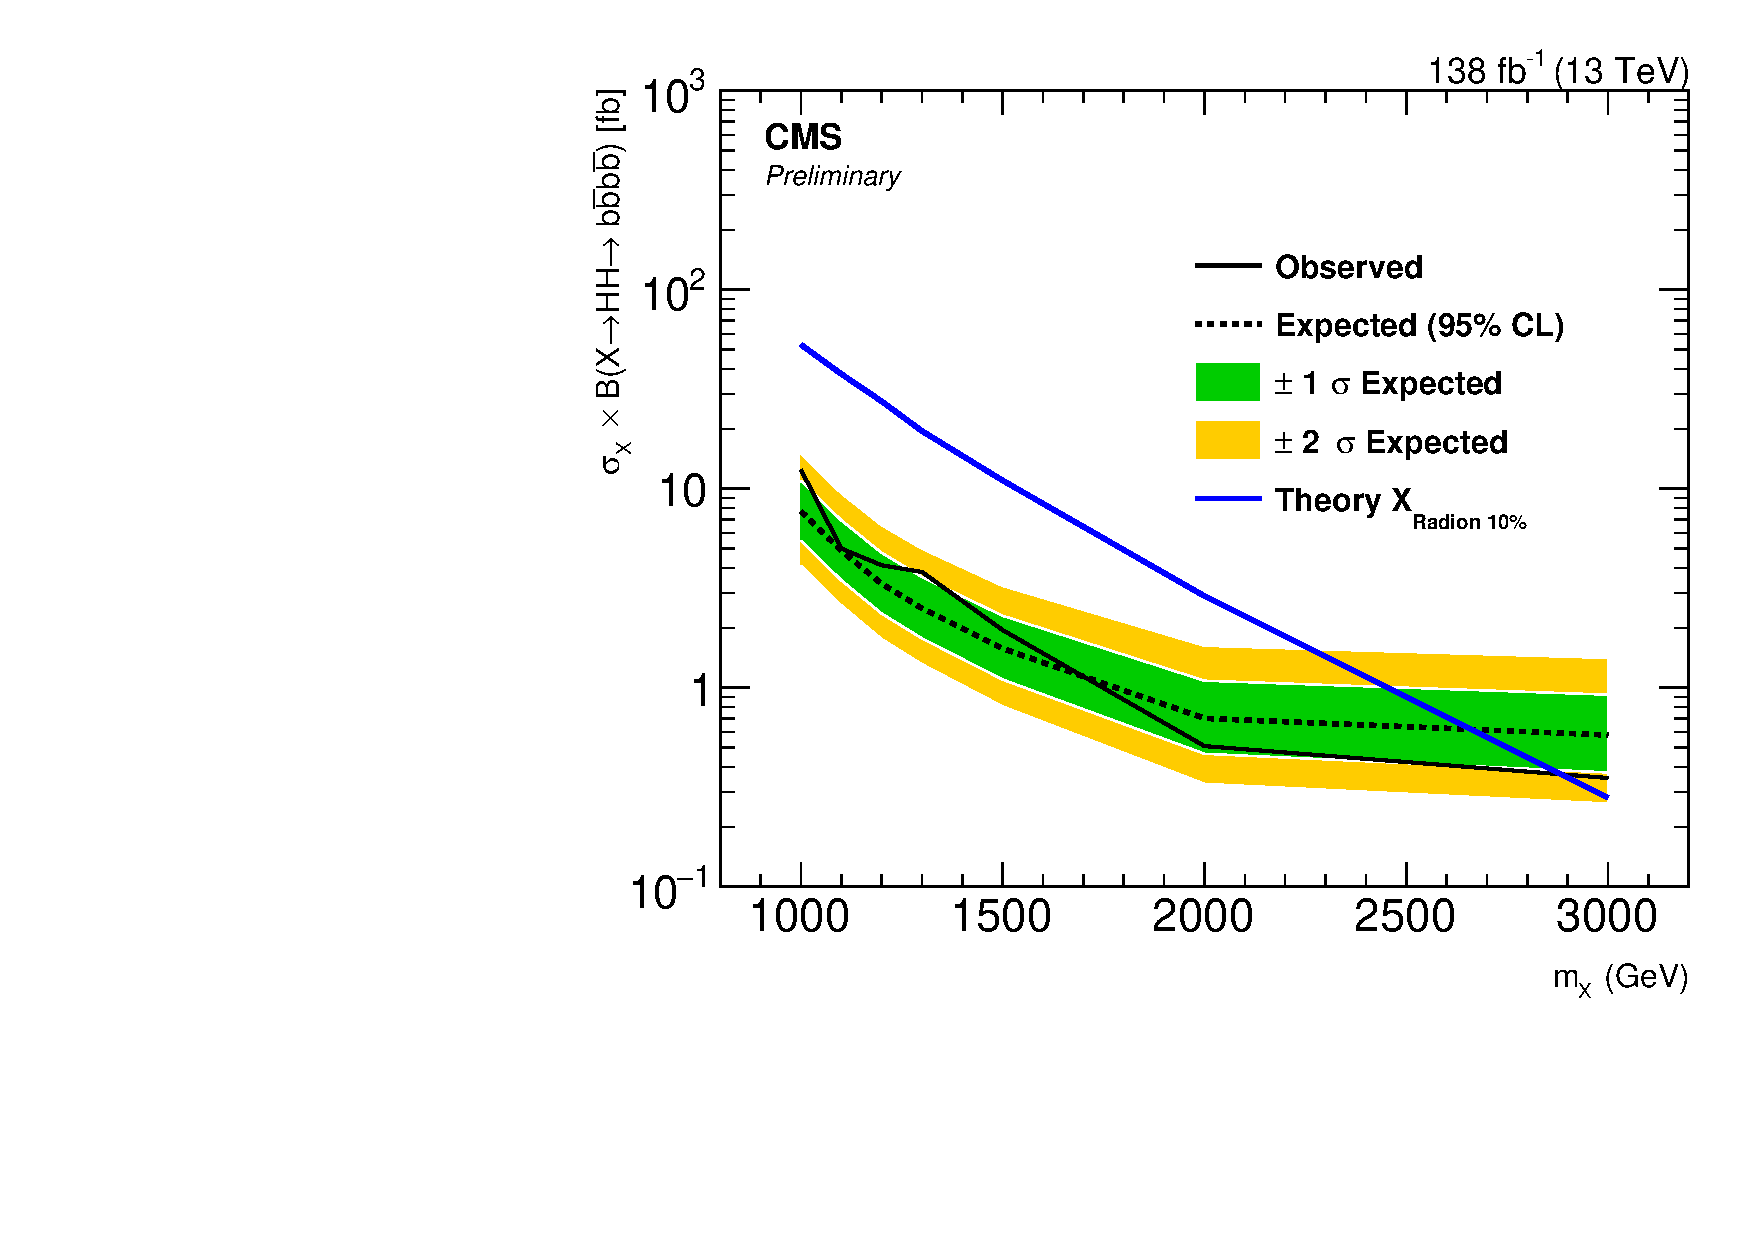
\includegraphics[width=0.45\textwidth]{Figures/limits_combine_137fb_dak8MDHbb_signalsAll_RadNarWIDE_2x2.pdf}
        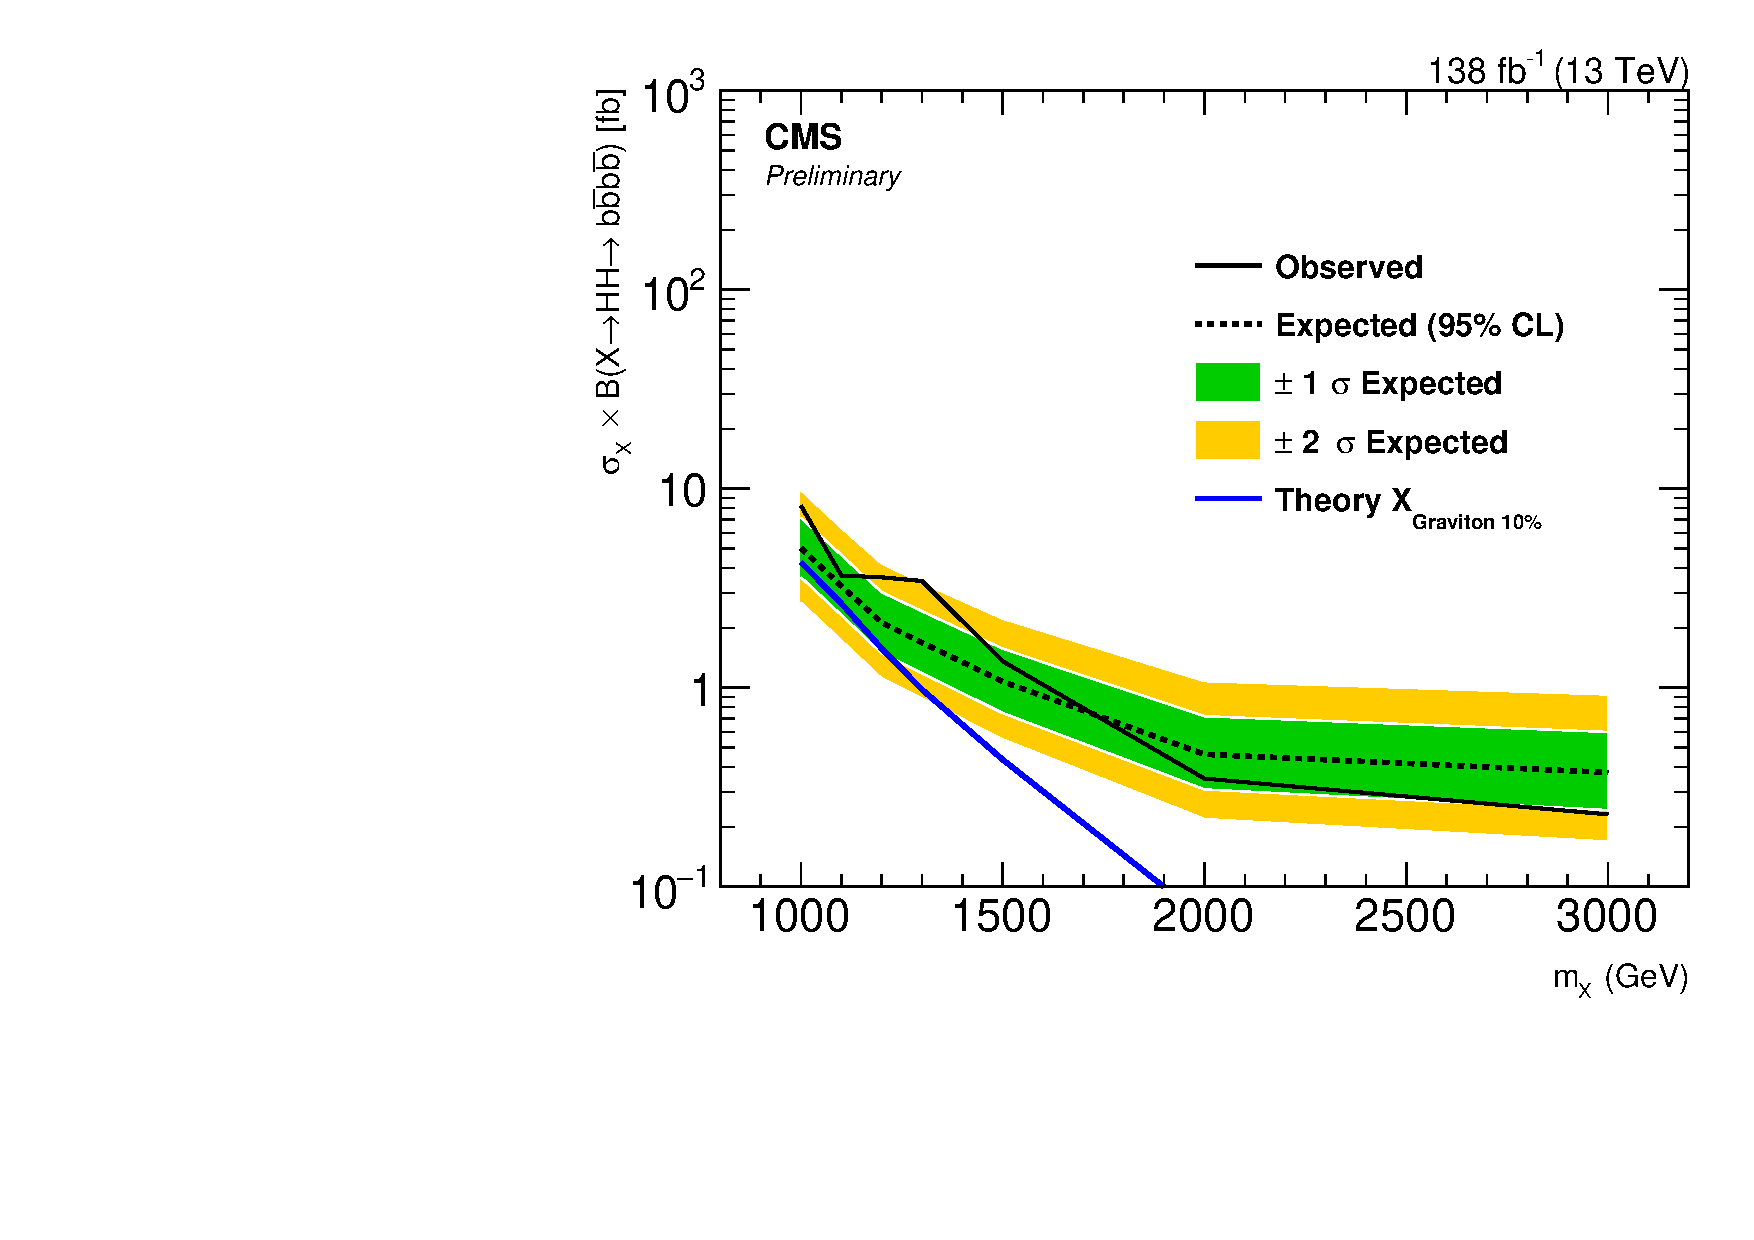
\includegraphics[width=0.45\textwidth]{Figures/limits_combine_137fb_dak8MDHbb_signalsAll_GravNarWIDE_2x2.pdf}
        \caption{Upper limits at 95\% confidence level on
        $\sigma(\Pp\Pp\to\PX) \mathcal{B}(\PX\to\bbbar\bbbar)$
        for the 10\% width spin-0 radion (left) and
        the spin-2 bulk graviton (right) models.}
	\label{fig:RadionLimitFULLWide}
 	\label{fig:GravitonLimitFULLWide}
\end{figure}

\begin{table}[h]
	\begin{center}
	\caption{10\%-width Radion observed 95\% CL exclusion limits. }
	\label{tab:ExpLimRadWide}
	\begin{tabular}{c c c c c c c } 
	 \hline
	   Mass& Obs. & Exp. lim.& $+$Exp (68\%)& $-$Exp (68\%)& $+$Exp (95\%)& $-$Exp (95\%)\\
	   (GeV) & (fb) & (fb) & (fb) & (fb)& (fb)& (fb) \\
	\hline
	 1000 & 12.48 & 7.70 & 10.96 & 5.47 & 15.00 & 4.10 \\
	 1100 & 5.01 & 4.88 & 6.94 & 3.47 & 9.50 & 2.59 \\
	 1200 & 4.13 & 3.33 & 4.76 & 2.36 & 6.57 & 1.76 \\
	 1300 & 3.82 & 2.51 & 3.60 & 1.77 & 5.00 & 1.31 \\
	 1500 & 1.95 & 1.57 & 2.30 & 1.10 & 3.25 & 0.80 \\
	 2000 & 0.51 & 0.70 & 1.08 & 0.47 & 1.63 & 0.33 \\
	 3000 & 0.35 & 0.58 & 0.92 & 0.37 & 1.41 & 0.26 \\ 
	 \hline
	\end{tabular}
	\end{center}
\end{table}
	
\begin{table}[h]
	\begin{center}
	\caption{10\%-width Graviton observed 95\% CL exclusion limits. }
	\label{tab:ExpLimBGWide}
	\begin{tabular}{c c c c c c c } 
	 \hline
	 Mass& Obs. & Exp. lim.& $+$Exp (68\%)& $-$Exp (68\%)& $+$Exp (95\%)& $-$Exp (95\%)\\
	 (GeV) & (fb) & (fb) & (fb) & (fb)& (fb)& (fb) \\
	\hline
	 1000 & 8.23 & 5.03 & 7.15 & 3.59 & 9.86 & 2.67 \\
	 1100 & 3.67 & 3.25 & 4.64 & 2.32 & 6.38 & 1.73 \\
	 1200 & 3.59 & 2.12 & 3.02 & 1.49 & 4.22 & 1.11 \\
	 1300 & 3.44 & 1.68 & 2.42 & 1.18 & 3.37 & 0.88 \\
	 1500 & 1.36 & 1.07 & 1.57 & 0.75 & 2.22 & 0.55 \\
	 2000 & 0.35 & 0.46 & 0.72 & 0.31 & 1.08 & 0.22 \\
	 3000 & 0.23 & 0.36 & 0.60 & 0.24 & 0.92 & 0.17 \\
	 \hline
	\end{tabular}
	\end{center}
\end{table}
